% !TEX root=/home/tavant/these/manuscript/src/manuscript.tex

\section{Elements of the 2D PIC-MCC simulations}
  \label{sec-elements}
  \subsection{Principe of the PIC-MCC simulations}
    \label{subsec-intro}
    The \ac{PIC} simulation models particles moving freely on a grid.
    The grid is used to compute the electric field, in the electrostatic approximation by solving the Poisson equation
    \begin{equation}
      \label{eq-poisson}
      \Delta \phi = - \frac{\rho}{\epsilon_0}
    \end{equation}
    where $\phi$ is the electric potential, $\rho$ is the charge density, and $\epsilon_0$ the vacuum permittivity.
    If the electrostatic approximation is not correct, one needs to solve the Maxwell equations.

    The particles move following the Lorenz forces
    \begin{equation}
      \label{eq-Lor}
      m \vec{a} = q \vect{E} + q \vec{v} \times \vec{B}
    \end{equation}
    with $m$ and $q$, the particle mass and electric charge, respectively.
    The numerical particles followed in the simulations correspond to $q_f$ physical particles, with
    \begin{equation}
      q_f = \frac{n V}{\Npc}
    \end{equation}
    with $n$ the particle density, $V$ the volume of a cell, and $\Npc$ the number of numerical particles in a cell.
    A large enough number of particles is needed in order to obtain physical results.
    Indeed, an insufficient number of particles leads to numerical heating \cite{ueda1994}.
    Usually, a minimum of 100 particles per cell are used, but recent results seem to encourage to use more particles \cite{janhunen2018}.

  \subsection{Monte Carlo collisions}

    In \ac{PIC} simulations, collisions between charged and neutral particles can be modeled by binary collision, but this approach is computationally costly.
    Instead, a Monte-Carlo algorithm can be used \cite{vahedi1995}.
    This approach is very efficient and allows scattering, momentum transfer, and ionization to be consistently modeled.
    The propellant used in \ac{HET} is \ac{Xe}.
    The cross-sections used for modeling \ac{Xe} or other gases collisions are taken from the {\sc LXCat} database project \cite{LXCat_web,pancheshnyi2012}.
    Unless otherwise stated, the elastic, inelastic scattering and ionization reactions listed in \cref{tab-reactXe} are used.
    The cross-section values are summarized in \cref{fig-xexsection}.

    \begin{table}[hbt]
      \ra{1.3}
      \centering
      \caption{Reactions for xenon used in the PIC simulations}
      \label{tab-reactXe}
      \begin{tabular}{@{}lll@{}}  \toprule
        Reaction & Threshold & Reference\\ \midrule
        {\it Elastic scattering} & &\\
        e + Xe = e + Xe   & --   & \cite{Lxcat_Xe,Lxcat_Xe2} \\
        {\it Excitation} & &\\
        e + Xe = e + Xe$^*$   & 8.315eV   & \cite{Lxcat_Xe,Lxcat_Xe2} \\
        e + Xe = e + Xe$^*$   & 9.447eV   & \cite{Lxcat_Xe,Lxcat_Xe2} \\
        e + Xe = e + Xe$^*$   & 9.917eV   & \cite{Lxcat_Xe,Lxcat_Xe2} \\
        e + Xe = e + Xe$^*$   & 11.7eV    & \cite{Lxcat_Xe,Lxcat_Xe2} \\
        {\it Ionization} & &\\
        e + Xe = e + Xe$^+$   & 12.13eV   & \cite{Lxcat_Xe,Lxcat_Xe2} \\
        \bottomrule
      \end{tabular}
    \end{table}



    \begin{figure}[hbt]
      \centering
      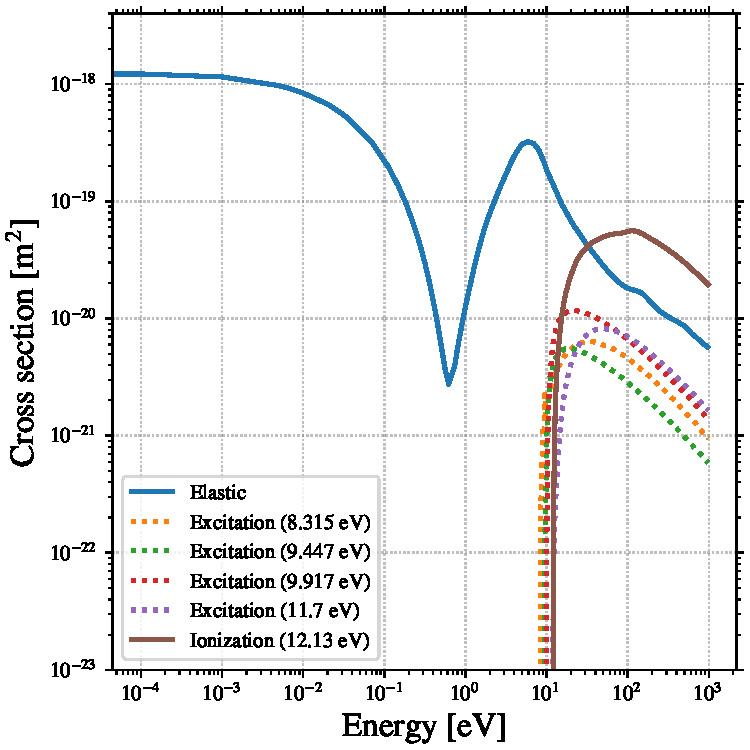
\includegraphics[width=\defaultwidth]{figure/xenon_cross_section.pdf}
      \caption{Cross section values used in the Monte Carlo procedure \cite{Lxcat_Xe,Lxcat_Xe2}.}
      \label{fig-xexsection}
    \end{figure}

    In the context of this thesis, and except precised otherwise, the `\ac{PIC} simulation' refers to the `\ac{PIC}-\ac{MCC} simulation'.
    In the case where no collision is modeled, we also call it `collisionless simulation'.
\section{Numerical implementation of the Particle in cell simulation}

  \LPPic is an explicit electrostatic \ac{PIC}-\ac{MCC} simulation code.
  Every time-step, the simulation loop presented in \cref{fig-picloop} is computed.
  The different steps constituting the PIC-loop are described in the next subsections.
  \begin{figure}[hbt]
    \centering
    \smartdiagramset{circular distance=4.5cm,
    module minimum width=3.5cm,
    text width=3cm,
    arrow tip=to}
    \smartdiagram[circular diagram:clockwise]{Particle Motion ,Boundary,Collision,Density weighting, Poisson Equation, Field weighting}
    \caption{\acs{PIC}-\acs{MCC} loop executed every time step.}
    \label{fig-picloop}
  \end{figure}


  \subsection{Computational characteristics}
    In \ac{PIC} simulations, there are two kinds of data used\string:
    \begin{itemize}
      \item Particles (electrons and ions; neutrals can be followed as well but not in \LPPic),
      \item Mesh, also named fields (densities, electric and magnetic fields, and so on).
    \end{itemize}


    \paragraph{Particles\\}
    For each particle, its position $\vec{x}$ and its velocity $\vec{v}$ are known.
    In most \ac{PIC}-\ac{MCC} simulations, the three directions of the velocity vector are followed in order to take into account scattering.
    It is abbreviated as \acs{3V}.
    The particle positions and velocity are not discretized, except to the numerical floating-point precision.

    One numerical particle represents a large number of physical particle. 
    Therefore they can be called \emph{superparticle} or \emph{macroparticle} in the literature.
    We will simply call them particle, unless the context require a precision.
    
    \paragraph{Fields\\}
    The fields are defined at the center of each cell of the mesh.
    The charge density $\rho$ is computed by depositing the particle on the mesh, using the Cloud-in-cell model \cite{birdsall1991}.
    The electric field at the position of the particle is also obtained by bilinear interpolation.
    The mesh dimension defines the dimension of the simulation.
    It is usual to find \acs{1D}\acs{3V} or \acs{2D}\acs{3V} \ac{PIC} simulations, for particles with 3 directions on the velocity but one (or two) dimensions in space.
    
    Early studies on the stability of the \ac{PIC} simulations gave conditions for the cell size and the time step as functions of the physical parameters \citep{birdsall1991,turner2013}
    \begin{align}
      \dt  \ope &\leq 0.2,  \label{eq-dt_limit} \\
      \dx &\leq 0.5 \lde, \label{eq-dx_limit}
    \end{align}
    where 
    \begin{equation} \label{eq-def_ope}
      \ope =  \sqrt{\frac{e^2 n_e}{ \epsilon_0 m_e}}
    \end{equation}
    is the electron plasma frequency, and 
    \nomenclature[Q]{\ensuremath{ \ope}}{  electron plasma frequency $\ope =  \sqrt{\frac{e^2 n_e}{ \epsilon_0 m_e}}$}
    \begin{equation} \label{eq-def_lde}
        \lde = \sqrt{\frac{ \epsilon_0 e\Te}{e^2 n_e}} 
    \end{equation}
    is the Debye length.
    We recall the relation $e \Te = k_B T_e$, with $T_e$ in Kelvin and $\Te$ in volt.
    \footnote{The Debye length usually refers to the spatial scale over with a charge is screened by the other charged particles. }
    The conditions \ref{eq-dt_limit} and \ref{eq-dx_limit} can be combined to produce 
    \begin{equation} \label{eq-CFL}
      \frac{\dt}{\dx}\sqrt{\frac{e \Te}{m_e}} \leq 0.4,
    \end{equation}
    which can be seen as a constraint on the thermal electron velocity that must be much less than one cell per time step.
    Hence, condition \ref{eq-CFL} is usually referred as the Current condition.
    
    As presented before in \cref{subsec-intro}, a third condition applies on the ratio between the superparticle density and the physical particle density. 
    No universal rule exist, as a wide range of values may be appropriate to different context \citep{turner2006,turner2013}.
    A general consensus in low temperature plasma agree on using approximately 100 numerical particles per cell.
    
    \subsection{Memory requirement}
    Because of the particle discretization, the memory requirement for \ac{PIC} simulation can be tremendous.
    For instance, we estimate here the numerical parameters of a \ac{2D} \ac{HET} simulation.
    With a density $n_e = \sn{3}{17}\,\per\meter\cubed$, and an electron temperature $\Te=20\,\volt$, the Debye length is $\lde=\sn{6}{-5}\,\meter$.
    The simulation of a square domain of $2\,\centi\meter$ aside needs a mesh of approximately 650 cells in each direction, hence more than $\sn{4}{5}$ cells in total.
    With 100 electrons and 100 ions per cell, it is 85 million particles that are simulated.
    
    For every particles, we need to store at least the two values of position and the three values of velocity, thus 6 real number.
    Using the double-precision floating-point format, it corresponds to approximately 400 bits per particles.
    In total, around 33 billion bits, or 4 Go (gigaoctet) are needed to store the particle ! 
    To give a reference to the reader, a modern laptop has a RAM of 8 Go.
    Adding a thirst dimension of size 2 cm increases the number of cells to 300 millions, and the memory requirement for the particles to 2.5 Terabytes of memory.
    
    
    \subsection{Particle pusher}
    The interaction of the movement equation \cref{eq-Lor} is different for magnetized and non-magnetized particles.
    For non-magnetized particles, we use the leapfrog scheme \cite{birdsall1991}
    \begin{align}\label{eq-leapfrog}
      \vect{v}^t &= \vect{v}^{t-1} + \frac{q}{m} \vect{E} \dt, \\
      \vect{x}^t &= \vect{x}^{t-1} + \vect{v}^t \dt,
    \end{align}
    with the superscript $t$ designing the time step, $q$ and $m$ the particle electric charge and mass, $\vect{E}$ the electric field at the particle position, and \dt the time step duration.

    It is important to note that the leapfrog induces a shift of $\frac{\dt}{2}$ between the position and the velocity, as illustrated in \cref{fig-leapfrog}.
    \begin{figure}[hbt]
      \centering
      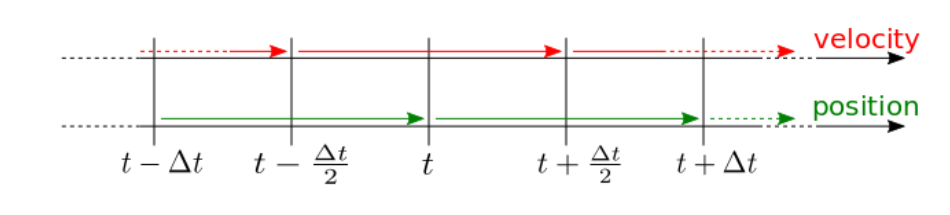
\includegraphics[width=\defaultwidth]{leapfrog.png}
      \caption{Illustration of the shift between the particle velocity and position.}
      \label{fig-leapfrog}
    \end{figure}
    This shift can lead to erroneous diagnostics when computing moments of the particles distribution.
    For instance, the mean velocity of an ensemble of $N$ particles at the instant $t$ is computed as\string:
    \begin{equation} \label{eq-meanv}
      \mean{\vect{v}}^t = \frac{1}{N} \sum_i^N \lp \vect{v_i}^t + \frac{q}{m} \vect{E_i} \frac{\dt}{2} \rp.
    \end{equation}
    Other moments like the mean energy or heat flux follow the same correction.
    We can see that the error between $\mean{\vect{v}}$ defined above and
    $$ \tilde{\vect{v}} = \frac{1}{N} \sum_i^N  \vect{v_i}^t $$
    is
    $$ \mean{\vect{v}} - \tilde{\vect{v}} =\frac{q \dt}{2 m}  \frac{1}{N}  \sum_i^N  \vect{E_i} .$$
    Hence, the error in the diagnostic is larger in the region of large electric field (as in the sheaths).

    \paragraph{Magnetized particles}
    For magnetized particles, we use a modification of the leapfrog algorithm proposed by Boris \cite{boris1970}.
    It corresponds to an operator splitting between the electrostatic acceleration and the magnetic rotation.
    This splitting is described below\string:

    \begin{enumerate}
      \item accelerate the particle during $\frac{\dt}{2}$\string: $\vect{v}^{t-\frac{\dt}{2}} = \vect{v}^{t-1} + \frac{q}{m} \vect{E} \frac{\dt}{2}$
      \item rotate the particle velocity with the magnetic field
      \item accelerate the particle during $\frac{\dt}{2}$\string: $\vect{v}^t = \vect{v}^{t-\frac{\dt}{2}} + \frac{q}{m} \vect{E} \frac{\dt}{2}$
    \end{enumerate}


  \subsection{Poisson equation solver}
  \label{subsec-poissonintro}

    In order to compute the electric field due to the particle charge density, the Poisson equation \cref{eq-poisson}  needs to be discretized over the mesh.
    We can directly discretize the differential operator by using the finite volume approach over a cell of the mesh.
    The formal discretization is developed in \cref{sec-diel}, for the particular case of taking into account the presence of dielectric boundaries.

    In \ac{1D}, the obtained linear system is tridiagonal.
    It can be solved directly using {\sc Thomas}' algorithm, which stores the Gauss elimination's coefficient.
    In \ac{2D}, the linear system is pentadiagonal.
    A direct solver, like the $LU$ decomposition, would require a large amount of memory to store the factorization matrices.
    On the other hand, as the time step is usually small in \ac{PIC} simulation, we expect the plasma potential $\phi$ not to change rapidly.
    Hence, an iterative solver using the previous solution as an initial guess seems more reasonable from both the memory storage and the computational time.
    The choice of the Poisson solver is discussed later in \cref{sec-lppic}.
    

    